\section{Physical rows and signed charge comparison}\label{sec:physical}

The finite-circle estimate of Section~\ref{sec:angular} is normalized
by a holomorphic scalar defined on a strip. We first show that this
scalar agrees asymptotically with the Perron normalization of physical
square-lattice rows. The proof combines a staggered finite matrix
calculation with the periodic six-vertex pressure. The disk-derived
screen estimates then identify square-plane limits of the reflected
diagrams and turn the matrix bounds into current estimates. Finally,
the passage and arm estimates control the signed boundary weights in
the charge comparison needed for the observable. Throughout this section,
\[
  \frac{\pi}{3}<\lambda<\frac{\pi}{2},\qquad
  d=2\cos\lambda\in(0,1),\qquad \rho=\frac{\lambda}{\pi}.
\]
Circumference limits are always taken with the lattice and every
insertion diagram fixed. Mesh limits are taken only afterwards.

\subsection{Staggered rows and their positive metric}
\label{physical:staggered-rows}

We use the functions $R,a,b,c,r,F$ of Section~\ref{sec:angular}, with
$\pi/3<\lambda<\pi/2$, $d=2\cos\lambda$, $\rho=\lambda/\pi$, and $v=\pi/2$.
The finite algebra and estimates below also hold throughout
$0<\lambda<\pi/2$.
In particular,
\begin{equation}\label{physical:F-identities}
 F(\overline u)=\overline{F(u)},\qquad
 F(\lambda-u)=F(u),\qquad F(u)F(-u)=r(u).
\end{equation}
The last identity continues $F$ to $-\lambda<\Re u<0$; reflection about
$\lambda/2$ continues it past the other edge. These continuations are
nonzero in the regions used below.

Put $\delta_*=\lambda/4$. For even $N$, let
$\mathcal H_N=(\C^2)^{\otimes N}$ and set
\begin{align}
 u_j(U)&=U+(-1)^{j+1}\delta_*,
 &\Phi(U)&=F(U+\delta_*)F(U-\delta_*),\label{physical:stagger-arguments}\\
 T_N^D(U)&=\Tr_p\bigl[D_pR_{p1}(u_1(U))\cdots R_{pN}(u_N(U))\bigr],
 &A_{N,\mathrm{stag}}^D(z)&=
 \frac{T_N^D(\rho(v-z))}{\Phi(\rho(v-z))^{N/2}}.
 \label{physical:staggered-transfer-definition}
\end{align}
The auxiliary space is indexed by $p$ and has dimension two. Let $P_{12}$
denote the exchange of two spin factors, and define
\begin{equation}\label{physical:metric}
 C=P_{12}R_{12}(\lambda/2),\qquad
 G_N=\prod_{j=1}^{N/2}C_{2j-1,2j},\qquad
 \langle x,y\rangle_{G_N}=x^*G_Ny.
\end{equation}
Norms and adjoints relative to this inner product are denoted by
$\|\cdot\|_{G_N}$ and $*G_N$. The four eigenvalues of $C$ are
$a_*,a_*,1+a_*,1-a_*$, where
$a_*=a(\lambda/2)=b(\lambda/2)=1/(2\cos(\lambda/2))<1$.
Thus $G_N$ is positive definite. Its condition number need not be bounded
as $N$ grows; the estimates below are proved directly in this inner product.

\begin{lemma}[Exchange, adjoint, and strip bound]
\label{physical:exchange-adjoint}
For $x-y=\lambda/2$ one has
\begin{equation}\label{physical:pair-exchange}
 C_{12}R_{p1}(x)R_{p2}(y)C_{12}^{-1}
   =R_{p1}(y)R_{p2}(x).
\end{equation}
For $K(\zeta)=\operatorname{diag}(\zeta,\zeta^{-1})$, $|\zeta|=1$, put
$P_{N,\zeta}^{\mathrm{stag}}=A_{N,\mathrm{stag}}^{K(\zeta)}$.
The family with fixed $\zeta$ commutes and satisfies
\begin{equation}\label{physical:row-adjoint}
 \bigl(P_{N,\zeta}^{\mathrm{stag}}(z)\bigr)^{*G_N}
       =P_{N,\zeta}^{\mathrm{stag}}(-\overline z).
\end{equation}
It therefore has a common $G_N$-orthonormal eigenbasis. Moreover,
\begin{equation}\label{physical:uniform-strip-bound}
 \|A_{N,\mathrm{stag}}^D(z)\|_{G_N}\le 2\|D\|,
 \qquad -v\le\Re z\le v.
\end{equation}
The constant is independent of even $N$.
\end{lemma}

\begin{proof}
Multiply the Yang--Baxter identity on the two site spaces by their
exchange $P_{12}$. Since this exchange interchanges the site labels, the
result is~\eqref{physical:pair-exchange}; invertibility holds at
$x-y=\lambda/2$ by positivity of $C$.

We first record the adjoint calculation for arbitrary $D$. Let
$J=\left(\begin{smallmatrix}0&1\\1&0\end{smallmatrix}\right)$
reverse the two basis states of the single auxiliary spin, and put
$D^\sharp=J\overline D J$.
Taking the ordinary adjoint reverses the site order. Auxiliary transpose
reverses it back, because the entries belonging to distinct site spaces
commute. Applying
$J_pR(u)^{t_p}J_p=R(\lambda-u)$ gives a forward row with arguments
$\lambda-\overline{u_j(U)}$ and boundary matrix $D^\sharp$.
These arguments are the exchanged stagger at central argument
$\lambda-\overline U$. Applying~\eqref{physical:pair-exchange} on each
complete pair gives
\begin{equation}\label{physical:raw-adjoint}
 G_N^{-1}T_N^D(U)^*G_N
       =T_N^{D^\sharp}(\lambda-\overline U).
\end{equation}
Equation~\eqref{physical:F-identities} gives the same transformation for
$\Phi$. For a unitary diagonal twist $K(\zeta)^\sharp=K(\zeta)$, proving
\eqref{physical:row-adjoint}. The usual two-auxiliary Yang--Baxter
calculation applies with these fixed site offsets: the difference of the
two row arguments is the same at every site, and
$K(\zeta)\otimes K(\zeta)$ commutes with the auxiliary intertwiner.
Taking the auxiliary traces proves commutativity. The adjoint belongs to
the same commuting family, so the family consists of commuting normal
matrices in the $G_N$ inner product.

For the bound, take $\Re U=0$ and write $x=U+\delta_*$, $y=U-\delta_*$.
Then $\overline x=-y$ and $\overline y=-x$. For
$E=R_{p1}(x)R_{p2}(y)$, taking the transpose of the exchange identity
and using $R(t)R(-t)=r(t)\id$ gives
\begin{equation}\label{physical:unfused-boundary-unitarity}
 E^{*C}E=r(x)r(y)\id=|\Phi(U)|^2\id.
\end{equation}
The last equality follows by multiplying the four factors in
$|F(x)F(y)|^2$ and using~\eqref{physical:F-identities}.
The normalized pair is consequently unitary for the metric
$\id_p\otimes C$. Embedded in the full space, it is unitary for
$\id_p\otimes G_N$, since all other factors of $G_N$ act on disjoint sites.
The product over pairs has norm one. Auxiliary trace with $D$ costs at
most $2\|D\|$, proving the bound on $\Re U=0$.
Equation~\eqref{physical:raw-adjoint} proves it on $\Re U=\lambda$, because
$\|D^\sharp\|=\|D\|$.

For fixed $N$, each normalized matrix entry is bounded as
$|\Im U|\to\infty$: each $R$ factor grows at most as
$\exp(|\Im U|)$, while
$\log|F(U\pm\delta_*)|=|\Im U|+O(1)$, also on the continued portions by
\eqref{physical:F-identities}. The strip maximum principle applied to
matrix elements between $G_N$-unit vectors proves
\eqref{physical:uniform-strip-bound} throughout the strip.
\end{proof}

\subsection{Fusion and exponentially small errors}
\label{physical:staggered-fusion}

Use two auxiliary spins, denoted by $p$ and $q$. The invariant line
$\C(|+-\rangle+|-+\rangle)$ for
$R_{pj}(u)R_{qj}(\lambda+u)$ has scalar block $r(u)\id_j$.
On the three-dimensional auxiliary quotient, use the fixed rescaled
basis of~\eqref{angular:fused-blocks} and write
\begin{equation}\label{physical:quotient-Y}
 Y(u)=\frac{b(u)}{r(u)}\mathcal L(u).
\end{equation}
Thus the two unmixed entries of $\mathcal L$ equal $-a$, and its mixed
two-by-two blocks are
\begin{equation}\label{physical:quotient-blocks}
 \begin{pmatrix}c&\sqrt d\\-\sqrt d&-b\end{pmatrix},
 \qquad
 \begin{pmatrix}c&-\sqrt d\\\sqrt d&-b\end{pmatrix}.
\end{equation}
All similarities on this quotient depend only on the fixed parameter
$\lambda$, not on $N$.

\begin{lemma}[Staggered fusion bound]\label{physical:fusion-bound}
Put $\phi(U)=\tan(\pi U/(2\lambda))$,
$\alpha=\tan(\pi/8)$, and
\begin{equation}\label{physical:two-Blaschke-factors}
 B_+(U)=\frac{\phi(U)-\alpha}{1-\alpha\phi(U)},\qquad
 B_-(U)=\frac{\phi(U)+\alpha}{1+\alpha\phi(U)}.
\end{equation}
For $|\Re U|<\lambda/2$, the normalized fused quotient product satisfies
\begin{equation}\label{physical:fused-error}
 \left\|\prod_{j=1}^NY_j(u_j(U))\right\|_{G_N}
 \le C_\lambda |B_+(U)B_-(U)|^{N/2}.
\end{equation}
The norm includes the fixed Euclidean norm on the quotient auxiliary
space. In particular the right side tends to zero uniformly on every
compact subset of this strip.
\end{lemma}

\begin{proof}
Applying~\eqref{physical:pair-exchange} to each auxiliary row separately,
and commuting factors acting on disjoint tensor factors before and after
each application, exchanges the arguments in a pair of fused site
matrices. The invariant line is in the auxiliary spaces, so this identity
passes to the quotient. The scalar product $r(x)r(y)$ is unchanged by
exchange. Hence, for $x-y=\lambda/2$,
\begin{equation}\label{physical:fused-pair-exchange}
 C_{12}Y_1(x)Y_2(y)C_{12}^{-1}=Y_1(y)Y_2(x).
\end{equation}

We give the reflected inversion identities needed at the two edges.
Let $Z(u)=Y(u)^{t_{\rm aux}}$, where the transpose is in the rescaled
three-dimensional auxiliary basis. Direct multiplication of
\eqref{physical:quotient-blocks} gives the meromorphic identities
\begin{equation}\label{physical:quotient-reflections}
 Y(u)^TY(-\lambda-u)=\id,
 \qquad Z(u)^TZ(\lambda-u)=\id.
\end{equation}
Here $T$ transposes both auxiliary and site indices. For completeness,
if $w=-\lambda-u$, then $b(w)=-c(u)$, $c(w)=-b(u)$, and
$a(u)a(w)=d-b(u)c(u)$. A mixed block of $\mathcal L(u)^T\mathcal L(w)$
therefore equals $(d-bc)\id$; the product of the scalar factors
$b/(ac)$ is $1/(a(u)a(w))$. The unmixed entries of $Y(u)$ and $Y(w)$
are $-b/c$ and $-c/b$. This proves the first identity.
For $w=\lambda-u$, one has $a(w)=b(u)$, $b(w)=a(u)$, and
$c(u)c(w)=d+a(u)b(u)$. After a fixed reordering, the mixed blocks of
$\mathcal L^{t_{\rm aux}}$ have diagonal entries $(-a,-b)$ and opposite
off-diagonal entries $\pm\sqrt d$. Their transpose products equal
$(d+ab)\id$, canceled by the scalar product $1/(c(u)c(w))$; the
unmixed entries are $b/a$ and $a/b$. This proves the second identity.

Write $Q(U)=Y_1(U+\delta_*)Y_2(U-\delta_*)$ and
$Q_s(U)=C Q(U)C^{-1}$. If $\Re U=-\lambda/2$, the first reflection in
\eqref{physical:quotient-reflections} interchanges the two arguments
after conjugation. Thus
\[
 Q(U)^*=Q_s(U)^{-1}=C Q(U)^{-1}C^{-1},
 \qquad Q(U)^{*C}Q(U)=\id.
\]
If $\Re U=\lambda/2$, put
$H(U)=Q(U)^{t_{\rm aux}}=Z_2(U-\delta_*)Z_1(U+\delta_*)$.
The order reversal is legitimate because entries on the two distinct
site spaces commute. Transposing the exchange identity gives
$C H(U)C^{-1}=Z_2(U+\delta_*)Z_1(U-\delta_*)$.
The second reflection identity now gives
$H(U)^*=(C H(U)C^{-1})^{-1}$, hence
$H(U)^{*C}H(U)=\id$.

The complete quotient product is therefore unitary in the metric
$\id_{\C^3}\otimes G_N$ on the left edge. On the right edge its auxiliary
transpose, a reversed product of these unitary pairs, is unitary.
Undoing a transpose in a three-dimensional tensor factor costs at most
three in operator norm. Indeed, its block-matrix expansion and
Cauchy--Schwarz give this bound; conjugation by $G_N^{1/2}$ commutes
with auxiliary transpose, so the same bound holds for the present norm.
The strip maximum principle yields a uniform bound in between.

There are no poles from $r(u_j(U))$ on this closed strip, since
$|\Re u_j(U)|\le3\lambda/4<\lambda$. Also $Y(u)$ has a scalar factor
$b(u)$ and hence vanishes at $u=0$. The complete product consequently
has a zero of order at least $N/2$ at each of $U=\delta_*$ and $U=-\delta_*$.
The two functions in~\eqref{physical:two-Blaschke-factors} have precisely
these zeros, modulus one on the strip edges, and modulus less than one
inside. Dividing the product by
$B_+(U)^{N/2}B_-(U)^{N/2}$ removes these zeros. For fixed $N$ the
quotient remains bounded at the two imaginary ends of the strip,
as follows directly from the trigonometric formulas. Applying the
maximum principle again proves~\eqref{physical:fused-error}.
\end{proof}

Fix $\epsilon\in\{-1,1\}$ and unit twists with
$\zeta/\xi=-\exp(\ii\epsilon\lambda)$. As in the homogeneous estimate,
take either $D=|-\rangle\langle+|$, $\tau=\epsilon$, or
$D=|+\rangle\langle-|$, $\tau=-\epsilon$, and put
\begin{align}
 M_N^{\mathrm{stag}}(z)&=
    e^{\ii\tau\rho z}A_{N,\mathrm{stag}}^D(z),\label{physical:marker}\\
 \mathcal N_N^{\mathrm{stag}}(z)&=
 M_N^{\mathrm{stag}}(z)P_{N,\zeta}^{\mathrm{stag}}(z)
 +P_{N,\xi}^{\mathrm{stag}}(z)M_N^{\mathrm{stag}}(z).
 \label{physical:marker-sum}
\end{align}
In the next displays the superscript $\mathrm{stag}$ is omitted.
Taking the fused auxiliary trace yields
\begin{align}
 \|P_{N,\eta}(z)P_{N,\eta}(z-\pi)-\id\|_{G_N}
   &\le C_\lambda e_N(U),\quad \eta\in\{\xi,\zeta\},
   \label{physical:inversion}\\
 \|M_N(z)P_{N,\zeta}(z-\pi)
       +P_{N,\xi}(z)M_N(z-\pi)\|_{G_N}
   &\le C_\lambda |e^{\ii\tau\rho z}|e_N(U),
   \label{physical:marker-inversion}\\
 e_N(U)&=|B_+(U)B_-(U)|^{N/2},\qquad U=\rho(v-z).
 \notag
\end{align}
Here $|\Re U|<\lambda/2$. To verify the invariant-line contributions,
$K(\eta)\otimes K(\eta)$ acts as the identity on that line, while
\[
 D\otimes K(\zeta)+e^{-\ii\tau\lambda}K(\xi)\otimes D
\]
annihilates it by the stated relation between the twists. Moreover,
$F(u)F(\lambda+u)=r(u)$ follows from~\eqref{physical:F-identities}.
Thus the line contributes exactly $\id$ in~\eqref{physical:inversion}
and zero in~\eqref{physical:marker-inversion}; the quotient is bounded by
Lemma~\ref{physical:fusion-bound}. Preserving or annihilating the line
also makes its off-diagonal block disappear under the auxiliary trace.
The identities shifted by $\pi$ give the corresponding estimates near
the other edge of the main strip.

On either vertical edge, \eqref{physical:row-adjoint} identifies the two
factors in~\eqref{physical:inversion} as adjoints. They are consequently
asymptotically unitary, uniformly on compact edge intervals. Combining
this with~\eqref{physical:uniform-strip-bound} on truncated strips and
then letting the truncation height tend to infinity gives
\begin{equation}\label{physical:asymptotic-contraction}
 \limsup_{\substack{N\to\infty\\N\ \mathrm{even}}}
 \sup_{x\in[-v,v]}\|P_{N,\eta}^{\mathrm{stag}}(x)\|_{G_N}\le1.
\end{equation}
Indeed the harmonic measure of the two horizontal sides tends uniformly
to zero on the compact real segment; the real endpoints are already
controlled by the edge estimate.

\subsection{Damping at the physical angles}
\label{physical:physical-damping}

\begin{proposition}[Staggered angular estimate]
\label{physical:staggered-transfer}
\label{physical:finite-staggered}
Let $\gamma_0=\pi/4$. In the notation
\eqref{physical:marker}--\eqref{physical:marker-sum}, let $B_{\rm out}$
and $B_{\rm in}$ be fixed finite products of $\xi$-twist and
$\zeta$-twist rows, respectively, at real arguments in $[-v,v]$.
Suppose that each product includes at least $n\ge1$ rows at arguments
in $\{-\gamma_0,\gamma_0\}$. Uniformly for $x,y\in[-v,v]$,
\begin{align}
 \limsup_{\substack{N\to\infty\\N\ \mathrm{even}}}
 \|B_{\rm out}\mathcal N_N^{\mathrm{stag}}(x)B_{\rm in}\|_{G_N}
       &\le C_\lambda n^{-1+\rho},\label{physical:staggered-low}\\
 \limsup_{\substack{N\to\infty\\N\ \mathrm{even}}}
 \|B_{\rm out}\bigl(\mathcal N_N^{\mathrm{stag}}(x)
       -e^{\ii\tau(x-y)}\mathcal N_N^{\mathrm{stag}}(y)\bigr)
       B_{\rm in}\|_{G_N}
       &\le C_\lambda n^{-1-\rho}.
       \label{physical:staggered-high}
\end{align}
Immediately on either side of either marker sum one may insert a product
of an even number of the corresponding twist rows, at arbitrary real
arguments in $[-v,v]$. The products may differ between the two terms;
the constant may depend on a common bound for these additional counts.
Every finite setup is fixed before the limit in $N$ is taken.
\end{proposition}

\begin{proof}
The three changes from the homogeneous argument are the $G_N$ metric,
the damping basepoint $e^{\ii\gamma_0}$, and the two-zero fusion error
in~\eqref{physical:fused-error}. We give the analytic argument to track
these changes explicitly. All diagonalizations and projections
in this proof are orthogonal for $G_N$; no comparison with the original
Euclidean norm is used. Suppress the superscript $\mathrm{stag}$.

Map the open $z$ strip to the right half-plane by $w=e^{\ii z}$, using
the branch with $-v<\Re z<v$. In a common eigenbasis of a fixed twist,
let $f_N(w)$ be any eigenvalue. It is holomorphic and uniformly bounded.
The adjoint identity gives
$f_N(\overline w)=\overline{f_N(w)}$ and hence $f_N(1)\in\R$.
For a fixed small $s>0$ restrict to eigenvalues satisfying
$|f_N(e^{\ii\gamma_0})|\ge e^{-s}$.
Every sequence has a subsequence converging on compact subsets to a
nonzero holomorphic function $f$ with $|f|\le1$. Nonzeroness follows
at $e^{\ii\gamma_0}$, and the bound follows from the edge unitarity and
strip bound proved above. Schwarz--Pick between $e^{\ii\gamma_0}$ and
$1$ gives, with $\alpha=\tan(\gamma_0/2)<1$,
\begin{equation}\label{physical:damping-Schwarz-Pick}
 |f(1)|\ge\frac{e^{-s}-\alpha}{1-\alpha e^{-s}}
             \ge1-C_\lambda s.
\end{equation}
The first inequality is the elementary extremal modulus bound for a
disk of pseudohyperbolic radius $\alpha$ centered at $f(e^{\ii\gamma_0})$;
take $s$ small enough that $e^{-s}>\alpha$.
Thus a large eigenvalue at the physical angle is also close in modulus
to a real sign at the center.

The remaining continuation argument uses the same analytic facts as
Lemmas~\ref{angular:edge-continuation}--\ref{angular:low-band}.
We verify the correspondence before applying their proofs:
\begin{enumerate}[label=(\roman*)]
\item The fixed-twist rows are commuting normal holomorphic matrices
in the $G_N$ inner product, with adjoint reflection
\eqref{physical:row-adjoint} and the uniform strip bound
\eqref{physical:uniform-strip-bound}.
\item The two-row and marker inversion errors in
\eqref{physical:inversion}--\eqref{physical:marker-inversion} tend
uniformly to zero on compact subsets of the same edge bands
$0<\Re z<\pi$ and $-\pi<\Re z<0$ used in the homogeneous proof.
The two zeros in the fused error change its rate of convergence, not
these bands or the resulting identities.
\item The marker has the same growth factor $|w|^{\tau\rho}$, and
\eqref{physical:damping-Schwarz-Pick} bounds the limiting row modulus
at $w=1$ below by $1-C_\lambda s$.
\end{enumerate}
These are precisely the inputs to the scalar continuation and Laurent
estimates. All their finite matrix elements can be taken between
$G_N$-unit vectors: the proofs use only the indicated intrinsic norms,
not a bounded comparison between $G_N$ and the Euclidean metric.

Here are their consequences with the present spectral cutoff. Define
\[
 E_{\eta,N}(s)=
 \one_{\{|P_{N,\eta}(\gamma_0)|\ge e^{-s}\}},\qquad
 \eta\in\{\xi,\zeta\}.
\]
By the adjoint identity, the moduli at $\gamma_0$ and $-\gamma_0$
agree on every common eigenvector. The scalar limits on this low
subspace are zero-free off the positive real $w$ axis by inversion
and Hurwitz's theorem. Dividing by the analytic square root of the
two-row product gives modulus one on each strip edge; the reflected
half-disk estimate from Lemma~\ref{angular:edge-continuation} bounds
the continued eigenvalues and their inverses there. Thus the scalar
limits extend across the two imaginary rays.

For $\sigma=\sgn f(1)$, Schwarz--Pick based at $1$ gives
\begin{equation}\label{physical:radial-sign-bound}
 |f(r)-\sigma|\le C_\lambda s\max(r,r^{-1}),\qquad r>0.
\end{equation}
Consequently the half-annulus proof, with $C_\lambda s$ in place of
$s$, gives bounded inverses on
\begin{equation}\label{physical:low-band-annulus}
 c_0^{-1}s<|w|<c_0/s,\qquad \Re w\ge0,
\end{equation}
and the sign estimate
\begin{equation}\label{physical:unit-semicircle-sign}
 f(w)=\sigma+O_\lambda(s),\qquad |w|=1,\quad\Re w\ge0.
\end{equation}
The constants absorb this fixed rescaling of $s$. An offending-eigenvalue
subsequence would contradict these scalar estimates, so they hold in
limsup for the diagonal compressions
$p_{\eta,N}=P_{N,\eta}|_{\operatorname{ran}E_{\eta,N}(s)}$ as well.
For sufficiently small fixed $s$ and all large $N$, their center
values are nonzero by \eqref{physical:damping-Schwarz-Pick}; hence we
may refine each projection according to the sign of $P_{N,\eta}(0)$.
Further spectral restrictions preserve every estimate.

Compress the marker to
$m_N=E_{\xi,N}(s)M_NE_{\zeta,N}(s)$. On the left half of the annulus
its continuation is represented, at $-w$ with $\Re w>0$, by
\begin{equation}\label{physical:marker-continuation}
 -p_{\xi,N}(w)^{-1}m_N(w)p_{\zeta,N}(w)^{-1}.
\end{equation}
The marker inversion identity glues this expression to the physical
one across both rays, exactly as in
Lemma~\ref{angular:marker-continuation}. The inverse bounds control
its errors. For every sequence of pairs of $G_N$-unit test vectors,
Montel's theorem therefore gives a scalar subsequential limit on the
full annulus with $|m(w)|\le C_\lambda|w|^{\tau\rho}$. No products
of limiting operators on varying spaces are used.

Writing $m(w)=\sum_{j\in\Z}\beta_jw^j$, Cauchy's estimates give
$|\beta_j|\le C_\lambda(C_\lambda s)^{|j-\tau\rho|}$ and hence
\begin{equation}\label{physical:Laurent-modes}
 |m(w)|\le C_\lambda s^\rho,\qquad
 \frac{m(w)-m(-w)}2=\beta_\tau w^\tau
       +O_\lambda(s^{1+\rho}),\qquad
 |\beta_\tau|\le C_\lambda s^{1-\rho}
 \quad (|w|=1).
\end{equation}
On equal-sign blocks the marker sum is
$2\sigma\beta_\tau e^{\ii\tau x}+O_\lambda(s^{1+\rho})$;
on opposite-sign blocks its two terms cancel to order
$O_\lambda(s^{1+\rho})$. The arbitrary-unit-vector subsequence
argument therefore yields, uniformly for real $x,y\in[-v,v]$,
\begin{align}
 \limsup_N\|E_{\xi,N}(s)\mathcal N_N(x)E_{\zeta,N}(s)\|_{G_N}
       &\le C_\lambda s^{1-\rho},\label{physical:low-band-low}\\
 \limsup_N\|E_{\xi,N}(s)
   (\mathcal N_N(x)-e^{\ii\tau(x-y)}\mathcal N_N(y))
   E_{\zeta,N}(s)\|_{G_N}
       &\le C_\lambda s^{1+\rho}.
       \label{physical:low-band-high}
\end{align}
There are only four sign blocks. On each one, an additional bounded
even row product is $\id+O_\lambda(s)$ by
\eqref{physical:unit-semicircle-sign}. Its error times the marker
bound is $O_\lambda(s^{1+\rho})$. This proves the same estimates
with the allowed additional lists, even when the two terms use
different lists.

Finally decompose each side spectrally according to
$h_{\eta,N}=-\log|P_{N,\eta}(\gamma_0)|$, assigning value $+\infty$
at a zero. Use the band $(-\infty,n^{-1}]$, successive dyadic bands
up to a fixed sufficiently small $s_0$, and the remainder.
On a band with positive lower endpoint $t$, each damping row at either
physical angle has norm at most $e^{-t}$, since the two moduli agree.
Commutativity and~\eqref{physical:asymptotic-contraction} show that the
whole exterior product has limsup norm at most $e^{-nt}$ on that band;
on the first band use $1$. For any pair of small bands use
\eqref{physical:low-band-low} or~\eqref{physical:low-band-high} with $s$
the larger upper endpoint. The double dyadic sum is bounded by
$C_\lambda n^{-\beta}$ for $\beta=1-\rho$ or $1+\rho$, respectively:
after writing each upper endpoint as $2^j/n$, its summands are bounded
by $C_\lambda n^{-\beta}2^{\beta\max(j,k)}e^{-c(2^j+2^k)}$, with the
first band interpreted as having no exponential cost. Terms involving
a remainder are exponentially small in $n$, by the uniform strip bound
and damping at least $e^{-ns_0}$. This proves both assertions.
\end{proof}

\subsection{The two physical steps}
\label{physical:physical-steps}

At $z=\gamma_0$ the staggered arguments are $\lambda/2,0$; at
$z=-\gamma_0$ they are $\lambda,\lambda/2$. Write $R_*=R(\lambda/2)$,
and let the cyclic shift on the spin basis be
\[
 S|s_1,s_2,\ldots,s_N\rangle
   =|s_2,\ldots,s_N,s_1\rangle.
\]
For clarity define the unnormalized, untwisted physical rows by
\[
 \mathsf T_N(+)=T_N^{\id}(\lambda/4),\qquad
 \mathsf T_N(-)=T_N^{\id}(3\lambda/4).
\]

\begin{lemma}[Physical rows and Perron vectors]
\label{physical:physical-row-algebra}
The physical rows satisfy
\begin{equation}\label{physical:shift-metric-rows}
 \mathsf T_N(+)=S G_N,\qquad
 \mathsf T_N(-)=S^{-1}G_N.
\end{equation}
For an arbitrary auxiliary matrix $D$, the marked rows are physical
rows with a single seam-edge insertion:
\begin{equation}\label{physical:seam-insertion}
 \begin{aligned}
 T_N^D(\lambda/4)&=D_N\mathsf T_N(+),\\
 T_N^D(3\lambda/4)&=(JD^TJ)_1\mathsf T_N(-),
 \qquad J=\begin{pmatrix}0&1\\1&0\end{pmatrix}.
 \end{aligned}
\end{equation}
The subscript specifies the physical spin factor on which the matrix
acts, and $T$ denotes ordinary transpose. With the periodic seam
anchored in a fixed physical chart, sites $N$ and $1$ are its two
neighboring sites; the insertion support stays fixed as $N$ grows.
The untwisted rows $\mathsf T_N(+)$ and $\mathsf T_N(-)$ are mutually
adjoint for $G_N$, commute, and are normal.
Both preserve each total-spin sector and are primitive on that sector.
Let
$\Lambda_N=\|\mathsf T_N(+)\|_{G_N}=\|\mathsf T_N(-)\|_{G_N}$.
In every sector whose Perron eigenvalue equals $\Lambda_N$, there is a
unique positive $G_N$-unit vector $\Omega$; it satisfies
\begin{equation}\label{physical:Perron-shift-identities}
 S^2\Omega=\Omega,\qquad
 \mathsf T_N(\pm)\Omega=\Lambda_N\Omega,\qquad
 \Omega^*G_NS^{\pm1}=\Lambda_N\Omega^*.
\end{equation}
All other eigenvalues in such a sector have strictly smaller modulus.
The scalar normalization in~\eqref{physical:staggered-transfer-definition}
at either physical angle is $F(\lambda/2)^{N/2}$.
\end{lemma}

\begin{proof}
We verify the collapse directly in components. Spin labels take values
$\pm1$. The collapsed vertices have entries
\[
 R(0)_{p,d;q,c}=\one_{p=c}\one_{d=q},\qquad
 R(\lambda)_{p,d;q,c}=\one_{p=-d}\one_{q=-c}.
\]
At the square vertex the equality $a(\lambda/2)=b(\lambda/2)$ gives
\begin{equation}\label{physical:matching-kernel}
 (R_*)_{-c_0,d_0;-d_1,c_1}
       =C_{d_0,d_1;c_0,c_1}.
\end{equation}
Each identity follows by listing the six nonzero entries of $R$.
In the auxiliary trace use indices $p_0,p_1,\ldots,p_N=p_0$ so that
the site $j$ factor is $(R(u_j))_{p_{j-1},d_j;p_j,c_j}$.
For the positive step the even sites force
$p_{2j-1}=c_{2j}$ and $p_{2j}=d_{2j}$, giving, with cyclic indices,
\[
 (\mathsf T_N(+))_{d;c}
   =\prod_{j=1}^{N/2}
     (R_*)_{d_{2j-2},d_{2j-1};c_{2j},c_{2j-1}}
   =(G_N)_{S^{-1}d;c}.
\]
The last equality uses that $R_*$ commutes with exchange of its two
spin factors. For the negative step the odd sites force
$p_{2j-2}=-d_{2j-1}$ and $p_{2j-1}=-c_{2j-1}$; hence
\[
 (\mathsf T_N(-))_{d;c}
   =\prod_{j=1}^{N/2}
     (R_*)_{-c_{2j-1},d_{2j};-d_{2j+1},c_{2j}}
   =(G_N)_{Sd;c},
\]
by~\eqref{physical:matching-kernel}. All auxiliary labels are fixed in
these sums, so neither collapse introduces an additional cycle factor.
This proves~\eqref{physical:shift-metric-rows}.

For a general auxiliary insertion, leave the trace indices separate
and multiply by $D_{p_N,p_0}$. At the positive step the last collapsed
vertex has $p_N=d_N$, so this factor applies $D$ to the last output
spin of the untwisted row. At the negative step the first collapsed
vertex has $p_0=-d_1$. Comparing with an untwisted output spin
$\widetilde d_1$ gives the factor
$D_{-\widetilde d_1,-d_1}=(JD^TJ)_{d_1,\widetilde d_1}$.
These are the two identities in~\eqref{physical:seam-insertion}.

The product defining $G_N$ is invariant under translation by two sites,
so $[G_N,S^2]=0$. Consequently
\[
 (SG_N)^{*G_N}=S^{-1}G_N,\qquad
 SG_NS^{-1}G_N=S^{-1}G_NSG_N.
\]
This proves mutual adjointness, commutativity, normality, and equality of
the two norms.

The matrix $C$ preserves the number of positive spins, has positive
diagonal entries, and has a positive exchange entry on each unlike pair.
Thus a step of $SG_N$ can hold every complete pair or can exchange any
chosen subset of its unlike pairs, followed by the cyclic shift.
Over $N$ steps, holding all pairs gives the identity permutation. Holding
everywhere except for one chosen pair exchange gives any prescribed
adjacent transposition: the shifts before and after the exchange move
that complete pair to any desired cyclic bond. All the corresponding
weights are positive. Adjacent transpositions connect all configurations
in a fixed-spin sector, so $SG_N$ is irreducible there. The same argument
works with $S^{-1}G_N$.

There is also a one-step self-loop in every sector. For a sector with at
most $N/2$ positive spins, place them on odd sites and put negative spins
on every even site. Exchange each unlike complete pair before applying
$S$; the original configuration is recovered. For a sector with more
than $N/2$ positive spins, reverse all spins in this construction.
For $S^{-1}G_N$, reverse the roles of the two parities. These self-loops
and irreducibility prove primitivity.

Perron--Frobenius gives a unique positive ray in each sector and strict
modulus inequality for its remaining eigenvalues. Normality says that
the largest Perron eigenvalue over the sectors equals $\Lambda_N$.
The operator $S^2$ commutes with $SG_N$ and preserves positivity, so
uniqueness of the positive ray makes $S^2\Omega$ a positive multiple of
$\Omega$. Since $S^2$ has finite order, that multiple equals one.
It follows that $S^{-1}G_N\Omega=S^{-2}(SG_N)\Omega
=\Lambda_N\Omega$. Taking $G_N$ adjoints and then canceling the
invertible rightmost $G_N$ gives the last identity in
\eqref{physical:Perron-shift-identities}.
Finally, $F$ is positive on the real interval under consideration;
\eqref{physical:F-identities} gives $F(0)=F(\lambda)=1$.
Thus $\Phi(\lambda/4)=\Phi(3\lambda/4)=F(\lambda/2)$, as claimed.
\end{proof}

For later normalization arguments, the preceding lemma also identifies
the finite Schatten moments without a dimension factor. If
$\mu_1,\ldots,\mu_{2^N}$ are the eigenvalues of $\mathsf T_N(+)$, then
for even $M$,
\begin{equation}\label{physical:Schatten-moment}
 \Tr\bigl[(\mathsf T_N(+)\mathsf T_N(-))^{M/2}\bigr]
       =\sum_{j=1}^{2^N}|\mu_j|^M,
 \qquad
 \lim_{M\to\infty}
 \Tr\bigl[(\mathsf T_N(+)\mathsf T_N(-))^{M/2}\bigr]^{1/(NM)}
       =\Lambda_N^{1/N}.
\end{equation}
The expression on the left, raised to $1/(NM)$, decreases in even $M$
because the unnormalized $\ell^M$ norm of a finite vector decreases
with $M$.

For the remaining square-medium arguments we write \(G=G_N\) and
\(T_N^\pm=\mathsf T_N(\pm)\), keeping the circumference implicit
in the metric.

\subsection{The physical scalar divisor}

The six-vertex free-energy formula goes back to Lieb and Sutherland
\cite{Lieb1967FModel,Sutherland1967SixVertex}.  We use the rigorous
periodic theorem of Duminil-Copin, Kozlowski, Krachun, Manolescu, and
Tikhonovskaia~\cite[Theorem~1]{SixVertex2022} at the weights below, and
prove the further finite-row normalization needed for the current estimates.

Let \(a_*=\sin(\lambda/2)/\sin\lambda\). The six-vertex model with
paired weights \((a_*,a_*,1)\) has anisotropy
\[
 \Delta=\frac{2a_*^2-1}{2a_*^2}=-\cos\lambda\in(-1/2,0).
\]
The following use of the free-energy theorem concerns only periodic
six-vertex boxes, not a random-cluster scaling limit.

\begin{lemma}[The strip divisor and the periodic pressure]
\label{physical:pressure}
For the ordinary square-lattice six-vertex model at these weights,
the iterated periodic pressure per vertex is
\begin{equation}\label{physical:free-energy}
 f_* = \log a_*+
 \int_0^\infty
 \frac{\sinh((\pi-\lambda)t)\tanh(\lambda t)}
      {t\sinh(\pi t)}\,\dd t
 =\log F(\lambda/2),
\end{equation}
where \(F\) is the strip normalization of Section~\ref{sec:angular}.
In particular, a sequence of even periodic rectangles, with both
periods tending to infinity, attains this pressure.
\end{lemma}

\begin{proof}
Theorem~1 of \cite{SixVertex2022}, with its parameters
\[
 \zeta=\lambda,\qquad \theta=\pi/2,\qquad
 r=\frac1{2\cos(\lambda/2)},
\]
has exactly the paired weights \((a_*,a_*,1)\). Its disordered-regime
formula is the first expression in \eqref{physical:free-energy}:
the integral over the real line is even and its numerator at
\(\theta=\pi/2\) contains \(\sinh(\lambda t)\).
The theorem supplies the iterated cylinder pressure; choosing the
second period sufficiently large for each first period gives the
stated sequence. Restricting also the second period to even integers
does not change the cylinder Perron limit.

Here is the identification with \(F\), including its normalization.
The harmonic function
\[
 H(u)=\log|F(u)/a(u)|
\]
on \(0<\Re u<\lambda\) has zero data on the left edge and right-edge
data
\[
 g(y)=\log\left|\frac{\sin(\lambda+\ii y)}{\sin(\ii y)}\right|
 =\int_0^\lambda
 \frac{\sin(2\alpha)}{\cosh(2y)-\cos(2\alpha)}\,\dd\alpha.
\]
These statements follow from \(F(u)F(-u)=r(u)\), the reflection
symmetry of \(F\), and \(|a(\ii y)|^2=r(\ii y)\).
There is only a logarithmic singularity at the right-edge origin;
the imaginary growth is bounded after subtracting \(\log|a|\).
Exhaustion by rectangles therefore gives the strip Poisson solution.
For the Fourier transform convention
\(\widehat h(t)=\int_{\R}e^{-\ii ty}h(y)\,\dd y\), residue
integration on a rectangle of imaginary height \(\pi\) gives
\[
 \int_{\R}e^{-\ii ty}
 \frac{\sin(2\alpha)}{\cosh(2y)-\cos(2\alpha)}\,\dd y
 =\frac{\pi\sinh((\pi/2-\alpha)t)}{\sinh(\pi t/2)}.
\]
The poles are at \(\ii\alpha\) and \(\ii(\pi-\alpha)\);
the value at \(t=0\) is obtained by continuity. The multiplier from
right-edge data to the midpoint is \(1/(2\cosh(\lambda t/2))\).
Integrating in \(\alpha\) thus gives
\[
 H(\lambda/2)=\frac14\int_{\R}
 \frac{\cosh(\pi t/2)-\cosh((\pi/2-\lambda)t)}
 {t\sinh(\pi t/2)\cosh(\lambda t/2)}\,\dd t.
\]
Use the difference-of-cosines identity, replace \(t\) by \(2t\),
and use evenness. This is the integral in
\eqref{physical:free-energy}. Since both \(F(\lambda/2)\) and
\(a_*\) are positive, the asserted equality follows.
\end{proof}

\begin{proposition}[Vacuum normalization at every circumference]
\label{physical:vacuum-divisor}
Let \(T_N^+=SG\), \(T_N^-=S^{-1}G\) be the untwisted physical
rows on an even circle and set \(\Lambda_N=\|T_N^+\|_G\).
Then
\begin{equation}\label{physical:divisor-comparison}
 \Lambda_N\ge F(\lambda/2)^{N/2},\qquad
 \frac{\Lambda_N}{F(\lambda/2)^{N/2}}\longrightarrow1.
\end{equation}
Every fixed finite all-physical sandwich may consequently use one
divisor \(\Lambda_N\) per layer in place of the strip divisor,
without changing its operator-norm limsup bound in
Proposition~\ref{physical:finite-staggered}.
\end{proposition}

\begin{proof}
This proof compares finite row norms with the periodic pressure; it
does not use a plane limit.
For even \(N,M\), the physical indexed torus has partition function
\begin{equation}\label{physical:torus-moments}
 Z_{N,M}=\Tr\bigl((T_N^+T_N^-)^{M/2}\bigr)=Z_{M,N}.
\end{equation}
Every second indexed tile is a physical square.  On that parity, lifted
indices map to ordinary square coordinates by
\[
 (j,t)\longmapsto\left(\frac{j+t-1}{2},\frac{j-t-1}{2}\right),
\]
up to the choice of origin.  The other indexed tiles identify duplicate
spins with weight one.  Each collapsed time edge is incident to an
uncollapsed neighboring site, so no component consists only of duplicates
and no extra cycle factor remains.  The indexed periods become
\[
 \left(\frac N2,\frac N2\right),\qquad
 \left(\frac M2,-\frac M2\right).
\]
Their determinant has absolute value \(NM/2\), the number of physical
vertices.  Interchanging \(N,M\) reflects this ordinary torus.  Since
the physical weights have \(a=b\), that reflection proves the second
equality in \eqref{physical:torus-moments}, with all flux sectors retained.

The two rows commute and are each other's \(G\)-adjoints. If their
common eigenvalues are \(\alpha_j,\overline{\alpha_j}\), then
\[
 Z_{N,M}^{1/(NM)}=
 \left(\sum_j|\alpha_j|^M\right)^{1/(NM)}.
\]
The unnormalized finite-dimensional \(\ell^p\) norm decreases with
\(p\). Thus this expression decreases with even \(M\), and by
symmetry with even \(N\). Moreover,
\[
 \lim_{M\to\infty}Z_{N,M}^{1/(NM)}=\Lambda_N^{1/N}.
\]

Fix an ordinary periodic \(k\)-by-\(l\) rectangle. Among its seam
spin assignments, choose one carrying at least
\(2^{-2(k+l)}\) of its partition function. Repeating this same
assignment glues independent interiors of such rectangles.  If both
indexed periods are multiples of \(2\operatorname{lcm}(k,l)\), their
two physical period vectors lie in \(k\Z\times l\Z\).  The quotient
then contains exactly \(NM/(2kl)\) ordinary rectangles, whose opposite
seam assignments already agree.  Consequently, along this cofinal family,
\[
 Z_{N,M}^{1/(NM)}
 \ge \left(2^{-2(k+l)}Z^{\mathrm{ord}}_{k,l}\right)^{1/(2kl)}.
\]
For fixed even \(N_0,M_0\), choose such \(N\ge N_0\), \(M\ge M_0\).
Separate monotonicity bounds \(Z_{N_0,M_0}^{1/(N_0M_0)}\) below by the
same right side.  Letting \(M_0\to\infty\), and then letting \(k,l\)
grow along the sequence in Lemma~\ref{physical:pressure}, gives
\(\Lambda_{N_0}^{1/N_0}\ge F(\lambda/2)^{1/2}\) for every even \(N_0\).
The asymptotic contraction in \eqref{physical:asymptotic-contraction}
of the normalized staggered twist row,
applied to the untwisted physical step, gives the opposite inequality
in the limit for the ratio in \eqref{physical:divisor-comparison}.
Thus that ratio tends to one, not merely its \(N\)-th root.

The number of rows in each sandwich term is fixed while
\(N\to\infty\). Its products are bounded in the \(G\) norm and
the change of divisor is \(1+o(1)\) per row. This remains true when
the compared terms have different fixed row counts. Their difference
therefore changes by an error tending to zero.
\end{proof}

\subsection{From tori to the square plane}

\begin{proposition}[Local plane limits and marked ratios]
\label{prop:plane-limit}
For every fixed finite switch query, its law in ordinary square-lattice
domains converges whenever the distance from the query to the boundary
tends to infinity, uniformly over planar outer cap partitions.  These
limits define a unique square-plane switch law.  Ordinary and diagonal physical
six-vertex tori have the same limits for every fixed finitely
supported spin-insertion ratio, whenever both periods tend to
infinity. The periods need not have bounded aspect ratio.
Here a fixed insertion is a finite product of fixed matrices on
physical edges, or a finite linear combination of such products.
The torus trace is unrestricted in total spin; a twist winding around
a growing period is not a fixed insertion in this statement.
\end{proposition}

\begin{proof}
We first work exclusively in the plane. The screen and collar
estimates used here are Propositions~\ref{prop:screens}
and~\ref{prop:relative-collars}. Only full annuli are needed; they
have no bank classes, and the surrounding primal circuit determines
the boundary partition transmitted toward the query.
The bounded collar densities
and actual circuit screens of Propositions~\ref{prop:annular-density},
\ref{prop:screens}, and \ref{prop:relative-collars} give the following
uniform statement. For any fixed finite inner query, its conditional
law differs by a quantity tending to zero as the surrounding buffer
grows, uniformly over planar outside partitions.
Indeed couple a common positive part on an intermediate annulus.
With a probability bounded below, independent of the two outside
partitions, this common part contains an actual primal circuit.
Conditioning toward the inside, the circuit induces the same wired
boundary there. Iterating in separated collars contracts the range
of inner probabilities by a fixed factor, starting from bounded
density. Alternating primal and dual circuit screens also imply that
no raw strand meeting a fixed query escapes all large buffers.
This proves existence, uniqueness, self-duality, and lattice
symmetry of the planar local limit.

It is important not to apply a planar boundary estimate directly to
the exterior of a disk in a torus. Instead cut a fundamental chart
and remove \(O(N+M)\) seam edges and vertex identifications. The
remaining core is an ordinary plane graph. For any fixed core edge
configuration, restoring the seam changes its component count by
at most \(C(N+M)\). Summing over seam edge states changes its weight
relative to the free planar-core law by a factor between
\(\exp(-C(N+M))\) and \(\exp(C(N+M))\), also after normalization.
All constants depend only on the fixed model parameter.

In the winding expansion an oriented switch loop of total turn $W$
has factor $e^{\ii\rho W/2}$, with a common factor $a_*$ per physical
tile; the local orientation sum is $R(\lambda/2)$, as verified in
Lemma~\ref{physical:winding} below. A simple contractible loop has
turn $\pm2\pi$, while a simple essential loop has turn zero, by
isotopy to a straight essential cycle on the flat torus. Summing the
two orientations therefore gives loop weights $2\cos(\pi\rho)=d$
and $2$, respectively. To compare with torus FK,
thicken the open primal graph. If its total genus is \(g\), then
\(g\in\{0,1\}\), and its number of perimeter components is
\[
 |A|-|V|+2k(A)-2g.
\]
Thus the FK-to-loop discrepancy, apart from fixed factors, is the
bounded genus factor \(q^{-g}\) and the essential-loop tilt
\((2/d)^{\ell_{\mathrm{ess}}}\). Each essential strand has length
at least a constant times \(\min(N,M)\); disjointness gives
\[
 \ell_{\mathrm{ess}}\le C\frac{NM}{\min(N,M)}\le C(N+M).
\]
Consequently the complete unmarked spin-loop core law satisfies the
same pointwise density comparison with the free planar-core law:
\begin{equation}\label{physical:core-density}
 e^{-C(N+M)}\le
 \frac{\dd\mu_{N,M}^{\mathrm{tor,core}}}
      {\dd\mu_{N,M}^{\mathrm{pl,core}}}
 \le e^{C(N+M)}.
\end{equation}

We next obtain a stronger concentration bound under the planar
reference law. Let \(h\) be a bounded local switch statistic and
write \(\mu(h)\) for its plane mean. For a tolerance \(\eta>0\),
choose a fixed buffer size \(L\) so that every conditional mean
of an interior translate of \(h\), given the states outside its
buffer, is within \(\eta\) of \(\mu(h)\). This uses only planar
outside states. Color the translates into a fixed number
\(O(L^2)\) of classes having disjoint buffers. In one such class,
conditioning on any earlier values of \(h\) is a mixture of full
outside configurations for the next buffer. Its conditional mean
is therefore still within \(\eta\) of \(\mu(h)\). The elementary
bounded-variable exponential estimate, iterated over that class,
gives an exponential tail in the number of its translates.
Taking the union over the fixed color classes yields
\begin{equation}\label{physical:planar-concentration}
 \mu_{N,M}^{\mathrm{pl,core}}
 \left(\left|\overline h-\mu(h)\right|>3\eta\right)
 \le C_\eta e^{-c_\eta NM}
\end{equation}
for the average over translates outside the seam buffer.
The omitted strip contains \(O(L(N+M))\) translates. Its fraction
tends to zero whenever both periods grow. By
\eqref{physical:core-density}, the same deviation probability under
the torus law is bounded by
\(C_\eta\exp(C(N+M)-c_\eta NM)\), which tends to zero without an
aspect-ratio restriction. Translation invariance and boundedness
then give convergence of each unmarked local expectation.

Finally fix finitely many spin insertions. First take a large fixed
buffer containing them. The planar alternating-screen event in that
buffer has probability tending to one with its radius, and by the
unmarked local convergence the same is true on the torus. On that
event all raw strands meeting insertions are local. Summing their
orientations makes the insertion ratio a local function of the
switches. For \(m\) inserted edge matrices, at most \(m\) raw loop
components meet insertions, and breaking them at the marked edges
leaves at most \(2m\) oriented pieces. Summing their orientations
bounds the modified numerator by a constant depending on the fixed
matrices and \(m\). Their unmarked divisors are products of at
most \(m\) factors, each equal to \(d\) or \(2\), and are at
least \(d^m>0\). Thus the ratio is bounded uniformly in the torus
periods. This also treats off-diagonal insertions, including those
whose total spin change makes their contraction zero. The complement
of the screening event therefore has
arbitrarily small contribution. This proves the assertion for marked
ratios and for both slicings.

Fixed displacements of periods and finitely many changed positive
time steps in a balanced period alter only bounded-width seams;
the same proof applies. A long-time cylinder limit followed by a
circumference limit is realized by choosing each time period large
enough to approximate its finite-circumference vacuum coefficient.
The comparison above is applied along this joint sequence, never
with one period fixed.
\end{proof}

\subsection{Reflected ratios and the physical scalar estimate}

Let \(\mathcal S_N\) be the set of total-spin sectors whose Perron
eigenvalue is \(\Lambda_N\), and let \(\Omega_{N,\sigma}\) be the positive
\(G_N\)-unit Perron vector in sector \(\sigma\).  The physical rows are
primitive in each sector, so a long balanced cylinder selects the equally
weighted average over these vectors, with one divisor \(\Lambda_N\) per
physical layer.

We first specify the finite exterior networks whose averaged squared-norm
ratios have square-plane limits by Proposition~\ref{prop:plane-limit}.
At a fixed mesh, let \(\mathcal T_{\mathrm{in},N}\) and
\(\mathcal T_{\mathrm{out},N}\) be two fixed finite physical insertion
networks with \(m_{\mathrm{in}}\) and \(m_{\mathrm{out}}\) layers.  Their
layers are the square-medium steps \(\pm\pi/4\), and their inserted matrices
are supported on finitely many physical edges.  Read the future network
in its actual future orientation and define
\begin{equation}\label{physical:external-states}
 \begin{aligned}
 \psi_{\mathrm{in},\sigma,N}
 &=\Lambda_N^{-m_{\mathrm{in}}}\mathcal T_{\mathrm{in},N}\Omega_{N,\sigma},\\
 \psi_{\mathrm{out},\sigma,N}
 &=\Lambda_N^{-m_{\mathrm{out}}}
     \mathcal T_{\mathrm{out},N}^{*G_N}\Omega_{N,\sigma},\\
 R_{\mathrm{in},N}
 &=\frac1{|\mathcal S_N|}\sum_{\sigma\in\mathcal S_N}
      \|\psi_{\mathrm{in},\sigma,N}\|_{G_N}^2,\\
 R_{\mathrm{out},N}
 &=\frac1{|\mathcal S_N|}\sum_{\sigma\in\mathcal S_N}
      \|\psi_{\mathrm{out},\sigma,N}\|_{G_N}^2.
 \end{aligned}
\end{equation}
The adjoint in the future vector is the Hilbert-space representation of
the physical future covector.  Its algebraic factor \(G_N^{-1}\) is not
an additional local insertion.

Reflection in a diagonal cut, followed by complex conjugation and arrow
reversal, glues a lower state to its reflected upper state through \(G_N\).
For lower spins \((c_0,c_1)\) and upper spins \((d_0,d_1)\), the intervening
square has weight
\[
 (R_*)_{-c_0,d_0;-d_1,c_1}
 =(\operatorname{swap}R_*)_{d_0,d_1;c_0,c_1},\qquad R_*=R(\lambda/2).
\]
The upper zigzag is the next lower zigzag shifted by one, and
\begin{equation}\label{physical:left-vacuum}
 \Omega_{N,\sigma}^*G_NS^{\pm1}=\Lambda_N\Omega_{N,\sigma}^*.
\end{equation}
This is the left Perron equation from
\eqref{physical:Perron-shift-identities}; the two choices agree because
\(S^2\Omega_{N,\sigma}=\Omega_{N,\sigma}\).
For a past state \(\mathcal T\Omega_{N,\sigma}\) formed from \(m\) raw
layers, the reflected physical diagram therefore has numerator
\(\Lambda_N(\mathcal T\Omega_{N,\sigma})^*G_N
(\mathcal T\Omega_{N,\sigma})\) and divisor \(\Lambda_N^{2m+1}\).
The extra numerator factor cancels the extra reflected layer exactly,
leaving \(\|\Lambda_N^{-m}\mathcal T\Omega_{N,\sigma}\|_{G_N}^2\).
The future state has the same identity.  Averaging identifies each ratio
in \eqref{physical:external-states} with its finite reflected vacuum
coefficient.  A string on either side acts on that side's state; it does
not replace the matching kernel or commute through it arbitrarily.

For \(x\in\{-\gamma_0,\gamma_0\}\), \(\gamma_0=\pi/4\), define rows with
one vacuum divisor per physical layer by
\begin{equation}\label{physical:vacuum-rows}
 \widehat A_N^D(x)=\frac{T_N^D(\rho(v-x))}{\Lambda_N},\qquad
 \widehat P_{\eta,N}(x)=\widehat A_N^{K(\eta)}(x),\qquad
 \widehat M_N(x)=e^{\ii\tau\rho x}\widehat A_N^D(x),
\end{equation}
and put
\[
 \widehat{\mathcal N}_N(x)=
 \widehat M_N(x)\widehat P_{\zeta,N}(x)
 +\widehat P_{\xi,N}(x)\widehat M_N(x).
\]
The twists and marker convention are those of
\eqref{physical:marker}--\eqref{physical:marker-sum}.

\begin{theorem}[Physical scalar estimate]\label{thm:physical-transfer}
Fix an integer \(n\ge1\) and, at a fixed mesh, a finite physical-layer
setup as above.  All layer counts and all inserted edge matrices are fixed
before even \(N\to\infty\).  Let \(B_{\mathrm{out},N}\) and
\(B_{\mathrm{in},N}\) be products of the corresponding \(\xi\)- and
\(\zeta\)-twist rows in \eqref{physical:vacuum-rows}, each containing at
least \(n\) rows.  Every row is at a physical angle \(\pm\gamma_0\).

For \(x,y\in\{-\gamma_0,\gamma_0\}\), define either
\begin{align}
 \mathcal D_N^{\mathrm{low}}
 &=E_{\mathrm{out},N}\widehat{\mathcal N}_N(x)E_{\mathrm{in},N},
 \label{physical:physical-low-operator}\\
 \mathcal D_N^{\mathrm{high}}
 &=E^x_{\mathrm{out},N}\widehat{\mathcal N}_N(x)E^x_{\mathrm{in},N}
 -e^{\ii\tau(x-y)}E^y_{\mathrm{out},N}\widehat{\mathcal N}_N(y)
       E^y_{\mathrm{in},N}.
 \label{physical:physical-high-operator}
\end{align}
Each \(E\) is a separately even product of at most a fixed \(L\) physical
rows with the corresponding twist.  The lists for the two high terms may
differ, but the exterior networks in \eqref{physical:external-states}
are common to them.  Every row in these displays has its own divisor
\(\Lambda_N\).  Set, for \(a=\mathrm{low},\mathrm{high}\),
\begin{equation}\label{physical:averaged-scalar}
 \mathcal C_N^a=\frac1{|\mathcal S_N|}\sum_{\sigma\in\mathcal S_N}
 \left\langle\psi_{\mathrm{out},\sigma,N},
 B_{\mathrm{out},N}\mathcal D_N^a B_{\mathrm{in},N}
 \psi_{\mathrm{in},\sigma,N}\right\rangle_{G_N}.
\end{equation}
Then \(\mathcal C^a=\lim_{N\to\infty,\ N\ \mathrm{even}}\mathcal C_N^a\)
and \(R_{\mathrm{in}},R_{\mathrm{out}}\), the corresponding limits of
\eqref{physical:external-states}, exist.  They are the square-plane
scalar coefficient and its finite nonnegative reflected vacuum ratios.
They satisfy
\begin{align}
 |\mathcal C^{\mathrm{low}}|
 &\le C_{\lambda,L}n^{-1+\rho}
       \sqrt{R_{\mathrm{out}}R_{\mathrm{in}}},
 \label{physical:scalar-low}\\
 |\mathcal C^{\mathrm{high}}|
 &\le C_{\lambda,L}n^{-1-\rho}
       \sqrt{R_{\mathrm{out}}R_{\mathrm{in}}}.
 \label{physical:scalar-high}
\end{align}
The analogous fixed-diagram reflection across an ordinary tile-axis cut
gives the plane Cauchy--Schwarz inequality with its two reflected ratios.
\end{theorem}

\begin{proof}
At fixed \(N\), primitivity identifies the sector-averaged low coefficient,
or each of the two sector-averaged high coefficients separately, with the
long balanced-cylinder vacuum coefficient of its physical diagram.
Cauchy--Schwarz in \(G_N\), followed
by Cauchy--Schwarz in the finite sector average, gives
\[
 |\mathcal C_N^a|
 \le\|B_{\mathrm{out},N}\mathcal D_N^a B_{\mathrm{in},N}\|_{G_N}
       \sqrt{R_{\mathrm{out},N}R_{\mathrm{in},N}}.
\]
At either physical angle the strip divisor is \(F(\lambda/2)^{N/2}\).
Thus each row in \eqref{physical:vacuum-rows} is its normalized staggered
row multiplied by \(F(\lambda/2)^{N/2}/\Lambda_N\), which tends to one
by Proposition~\ref{physical:vacuum-divisor}.  Each row list is fixed
while \(N\) grows.  Proposition~\ref{physical:finite-staggered} therefore
gives the operator limsup \(C_{\lambda,L}n^{-1+\rho}\) or
\(C_{\lambda,L}n^{-1-\rho}\).  This use of the divisor comparison is
asymptotic, including when the two high terms have different row counts.

For each \(N\), choose one sufficiently large balanced time period that
approximates this finite set of vacuum coefficients: both scalar terms
in the high case and both reflected coefficients.  Proposition
\ref{prop:plane-limit} applies along the resulting joint sequence, since
\eqref{physical:seam-insertion} puts every row twist or marker on one
physical edge. The row counts and all other insertion supports are
fixed during this limit, so the diagrams have finitely supported
insertions and both periods tend to infinity. A twist on each of
finitely many such seam edges is covered by that proposition; no
insertion extends around a growing period. It identifies the limits
in the statement. In
particular the reflected limits are finite, and they are nonnegative as
limits of the norm squares in \eqref{physical:external-states}; this does
not assert positivity of individual winding summands.  Taking the limit
in the preceding Cauchy--Schwarz inequality proves the two bounds.

For an ordinary tile-axis cut, the untwisted homogeneous row at
\(u=\lambda/2\) is self-adjoint by \eqref{angular:normal-rows}.  Within
each spin sector its matrix has a positive diagonal and positive
transitions for adjacent unlike-spin exchanges, obtained by two auxiliary
exchanges; these connect the sector, so the row is primitive.  Reflection
matches the spin coordinates directly.  Using its own Perron divisor and
the ordinary Hilbert norm gives the same reflected finite identity and
sector-averaged Cauchy--Schwarz inequality.  The fixed-diagram plane limit
then gives the last assertion.
\end{proof}

The finite staggered proposition retains its arbitrary real spectral
arguments and arbitrary vector tests.  The plane theorem above concerns
only fixed physical-layer diagrams.  It allows finitely many seam matrices
on finitely many rows, but it supplies no plane interpretation for an
arbitrary sequence of \(G_N\) vectors, a nonphysical spectral row, or an
insertion winding around a growing period.  The row lists may grow in a
later mesh limit; they are fixed during each circumference limit.

For geometric current stencils, Proposition~\ref{prop:finite-extraction}
is the separate finite operator identity.  Its common-endpoint construction
uses four physical steps in the positive-time direction in each high term:
two marker-sum steps
and two unmarked before- or after-twist steps.  The common external tensors
and source phase follow from the finite tangency, tangent-lift, and ice
conservation identities.  Corollary~\ref{cor:finite-extraction-rates}
combines that identity with Theorem~\ref{thm:physical-transfer}.  Reflection
preserves \(\tau=1\), so its geometric high-stencil phase is unchanged.

\subsection{Winding weights and local caps}

We next evaluate the loop and boundary-arc weights that enter the
signed comparison. These identities are finite orientation sums. Put
\begin{equation}\label{physical:charges}
 \Delta_0=\frac{\pi}{2\lambda}-\frac32,\qquad
 s=\Delta_0+1,\qquad t=-\Delta_0,\qquad
 w(m)=\frac{\cos((m-\tfrac12)\lambda)}{\sin\lambda},\qquad
 Q=-e^{\ii\lambda}.
\end{equation}
Traverse a disk boundary with its interior on the left. At port \(i\),
let \(\theta_i\) be a lifted inward normal and let \(c=\pm1\)
denote the inward or outward spin. On an interval \(R\) with fixed
wire designation use
\begin{equation}\label{physical:boundary-factors}
 b_i(c)=(2\sin\lambda)^{-1/2}
 \exp\left\{\ii c\left(\frac{\rho\theta_i}{2}+\lambda h_i\right)\right\},
 \qquad h_i=H_R+\Delta_0\one_{\{i\text{ high}\}}.
\end{equation}
A port is high when the immediately preceding boundary gap has the
designated wire color. On a further lap the raw bases \(H_R\)
compensate the turn of the lifted normal, so the factors have the
prescribed periodicity.

\begin{lemma}[The two winding expansions]\label{physical:winding}
Orient the switch strands and give their turns the weights
\(\exp(\pm\ii\rho W/2)\). With the common coefficient \(a_*\)
for either switch, summing orientations gives the same real tensor
\(R(\lambda/2)\) for either global sign. Thus the two expansions
give identical finite contractions with arbitrary prescribed
boundary spin factors and edge insertions.

In the plus expansion a boundary disk arc, followed from its earlier
port \(i\) to its later port \(j\), has weight \(w(h_i-h_j)\).
For an even number of wire flips its two possible high statuses give
\begin{equation}\label{physical:even-flip-weights}
 w(g+\Delta_0)=\frac{\sin((2-g)\lambda)}{\sin\lambda},\qquad
 w(g-\Delta_0)=\frac{\sin((1+g)\lambda)}{\sin\lambda},
\end{equation}
where \(g\) is the raw base drop. An odd-flip arc has weight \(w(g)\).
The minus expansion has the same rule with
\(h_i\) replaced by \(-h_i-\theta_i/\pi\), and hence with the
complementary wire color defining high ports. A diagonal string of
charge \(a\) multiplies each crossing spin by
\(e^{\ii\lambda ac}\), where \(c\) is measured along its left
normal; its signed intersections shift the corresponding drops,
with the reverse convention in the minus expansion.
\end{lemma}

\begin{proof}
At a tile, the oriented tensor vanishes unless there are two incoming
arrows. For adjacent incoming arrows one pairing is allowed and its
two turns cancel. For opposite incoming arrows the two pairing
contributions sum to \(2\cos(\lambda/2)\). Multiplication by
\(a_*=1/(2\cos(\lambda/2))\) therefore gives the stated real
six-vertex tensor for both signs.

Close a boundary arc against its forward boundary interval, using
the normal endpoint tangents. Its turn is
\(\theta_j-\theta_i-\pi\). Multiplying its two boundary factors
by its plus winding weight and summing its two orientations gives
\(w(h_i-h_j)\); the lifted normal terms cancel. Reversing the
winding sign gives exactly the replacement
\(-h_i-\theta_i/\pi\). Ports inside the child interval pair
among themselves. Its endpoint high statuses are consequently
opposite for an even number of flips and equal for an odd number.
This proves the drop rules, and substitution of \(\Delta_0\)
gives \eqref{physical:even-flip-weights}. The string assertion is
the same orientation sum with its extra crossing factors.
\end{proof}

We call the plus expansion \emph{correct} and the minus expansion
\emph{wrong}; these names are kept when all wire colors are reversed.
A positive completion pairs successive high--low ports between
successive visits of the designated boundary color. The remaining
ports are completed planarly, ordinarily by wiring each primal
interval separately. Its completed-loop weight is \(d^\ell\).

\begin{lemma}[Local cap elimination]\label{physical:cap-elimination}
Fix finitely many designated boundary intervals, and consider a family
of boundary disk arcs closed under descendants, each with at most one
wire flip in its interval. Its cap-loop factors
are \(d\) for a zero-flip arc beginning high, and \(1\) for a
zero-flip arc beginning low or an arc containing one flip, up to
an aggregate factor \(d^{O(1+X)}\). Here \(X\) is the number of
unremoved arcs, or any passage count dominating their relevant
macroscopic portions. The implicit constant may depend on the fixed
number of designated intervals. The assertion holds for all \(d>0\).
\end{lemma}

\begin{proof}
Remove arcs from descendants outward, so the next two endpoints are
adjacent among the remaining ports. Joining them makes one completed
loop exactly when their exterior partners already pair them;
otherwise it reconnects those partners. Within a designated interval,
a high--low pair closes one cap loop and a low--high pair transports
the same local pattern. Across a flip the equal high statuses
transport an unmatched end without closing a loop. If two such
transported ends were already tied, the exceptional loop erases an
entire remaining designated interval. There are only boundedly many
whole-interval erasures. Other cap statuses are inherited unchanged.
At the end, each remaining arc accounts for at most a bounded number
of unremoved boundary loops. This proves the aggregate error.
Changing boundedly many extra ties changes the loop count by only
a bounded amount. No sign or positive corner-cost assertion is used.
\end{proof}

\subsection{The local costs}

Retain the flat-flip costs \(P\) and \(D_*\) of
Lemma~\ref{angular:flat-costs}. They are computed in fixed buffered
flat-wall charts at radius comparable to \(n\), measured in lattice
steps. Thus \(P\) is the logarithm of the probability of an actual
arm of the specified color from the gap, and
\(D_*=\log\EE d^{N_t}\), with \(N_t\) the raw local straddles
wholly inside its cutoff. For a bulk charge satisfying
\[
 0<a<1,\qquad (1+a)\lambda<\pi/2,
\]
define
\begin{equation}\label{physical:bulk-costs}
 u_\pm(a)=\frac{\cos((1\pm a)\lambda)}{\cos\lambda},\qquad
 F_\pm(a;R)=\EE\bigl[u_\pm(a)^{N(R)}\bigr],
\end{equation}
where \(N(R)\) counts the closed raw loops inside a buffered cutoff
of radius \(R\) that surround its bulk vertex. We write
\(F_\pm(a)=F_\pm(a;n)\) when the cutoff is comparable to \(n\).
All these weights are strictly positive. Fixed changes of cutoff
shape or scale, color, lattice symmetry, or allowed caps beyond the
buffer change their logarithms by \(O(1)\), by the bounded collar
densities of Lemmas~\ref{disk:initial-collars} and
\ref{disk:thin-collars} and the tilt estimates.  These bounded comparisons
count every bank-wire class meeting a chart, including a partial class;
their number is fixed by the local feature inventory, and the residual
rim caps are separately noncrossing.  Only bounded densities are used
for the mixed-bank flat-flip comparison. Separated local factors
compare in products by conditioning
on the other buffered patches. Proposition~\ref{prop:tilts} gives
polynomial absolute moments of every fixed power, logarithmic size
of the costs, and
\begin{equation}\label{physical:cutoff-increment}
 \left|\log F_\pm(a;n)-\log F_\pm(a;n^{1-\varepsilon})\right|
 \le C\varepsilon\log n+C.
\end{equation}
The flat-flip bounds are
\begin{equation}\label{physical:flip-costs}
 P\le-c_1\log n+C,\qquad
 D_*\ge P+c_2\log n-C,
\end{equation}
by Lemmas~\ref{angular:flat-costs} and~\ref{lem:strict-flip},
respectively. The region-tree path/cut alternative
identifies absence of local straddles with an actual gap arm after
a fixed cutoff enlargement, so either version gives these costs.

We use \(o(\log n)\) in one-sided inequalities to mean an allowance
\(\eta\log n+C_\eta\) for every \(\eta>0\). Here is the
elementary absorption rule used below. If \(X\) has all fixed
exponential moments uniformly bounded and \(V\) has all fixed
absolute moments bounded by powers of \(n\), then the contribution
of \(V\) on \(X>\delta\log n\) is smaller than any prescribed
inverse power of \(n\). Indeed Cauchy--Schwarz and
\(\PP(X>x)\le \EE e^{LX}e^{-Lx}\) prove this after choosing
\(L\). On the complement, \(C^X\le n^{\delta\log C}\) and
\(C^{-X}\ge n^{-\delta\log C}\). Thus such factors cost only
\(o(\log n)\) relative to a baseline bounded below by an inverse
polynomial. The same rule preserves a fixed polynomial saving if
\(\delta\) is chosen smaller than that saving.

\subsection{A charged cylinder below unit loop weight}

The transfer estimate now has the correct physical normalization.
To use it for the observable, we also need to control the sign of
boundary terms. The next inequality is obtained separately, by comparing
the two finite winding expansions of one cylinder and using the passage
and arm estimates. Its arm cost and positive nest factor are both
retained; these are the factors that enter the observable's error bound.

\begin{theorem}[Charge budget]\label{thm:charge-budget}
For any fixed finite list of charges satisfying
\[
 a_j>0,\qquad (1+a_j)\lambda<\pi/2,\qquad \sum_j a_j=1,
\]
for every \(\eta>0\) there is \(C_{\eta,\mathbf a}<\infty\) such that the
local costs obey
\begin{equation}\label{physical:charge-budget}
 P+D_*+\sum_j\log\frac{F_-(a_j)}{F_+(a_j)}
 \le \eta\log n+C_{\eta,\mathbf a}.
\end{equation}
The assertion is valid for either global wire designation, with
the fixed buffered cutoff conventions just specified.  Equivalently,
the left side has the one-sided \(o(\log n)\) allowance defined above.
\end{theorem}

\begin{proof}
Fix \(0<\varepsilon<1/2\) and put \(r=n^{1-\varepsilon}\).
Use a straight cylinder with even circumference comparable to \(n\)
and height \(Kn\log n\), where \(K\) will be fixed sufficiently
large. Place two bottom flips, named \(s\) and \(t\), a distance
of order \(n\) apart, and no top flips. The same letters denote
their effective drops from \eqref{physical:charges}. All bulk
endpoints \(z_j\) are grouped near the \(s\)-gap: their heights,
pairwise separations, and distances from that gap are comparable to
\(r\). Give them disjoint cutoff boxes and larger buffers of small
fixed fractions of \(r\), leaving clear corridors around them.
The \(t\)-cutoff is a small fixed fraction of \(n\).

Choose the two positive cap completions as a paired choice under
global color reversal, including any residual planar ties. Thus
reversing every designation exchanges the two completed switch laws
exactly; it does not change the cylinder or its tile weights.

Draw strings of charges \(-a_j\) from the \(s\)-gap to \(z_j\).
Use raw bottom drops \(s-1,t\), whose sum is zero, and constant
raw base on top. An oriented intersection shifts a correct disk
drop by \(+a_j\) if its interval contains the launch and by
\(-a_j\) if its disk contains the endpoint. Thus the local
effective drops are \(s,t\). In the wrong expansion they are
\(-s,-t\), with the enclosed endpoint charge added.
Figure~\ref{fig:charged-cylinder} records the cylinder and the
separate arm requirements used below.

The comparison must keep the local positive weights on the same
events throughout the proof. In particular, the possibly small factor
from raw straddles at the distant flip will multiply both the positive
main event and the exceptional event carrying a negative term. A
saving only for their unweighted probabilities would not suffice.

\begin{figure}[tbp]
\centering
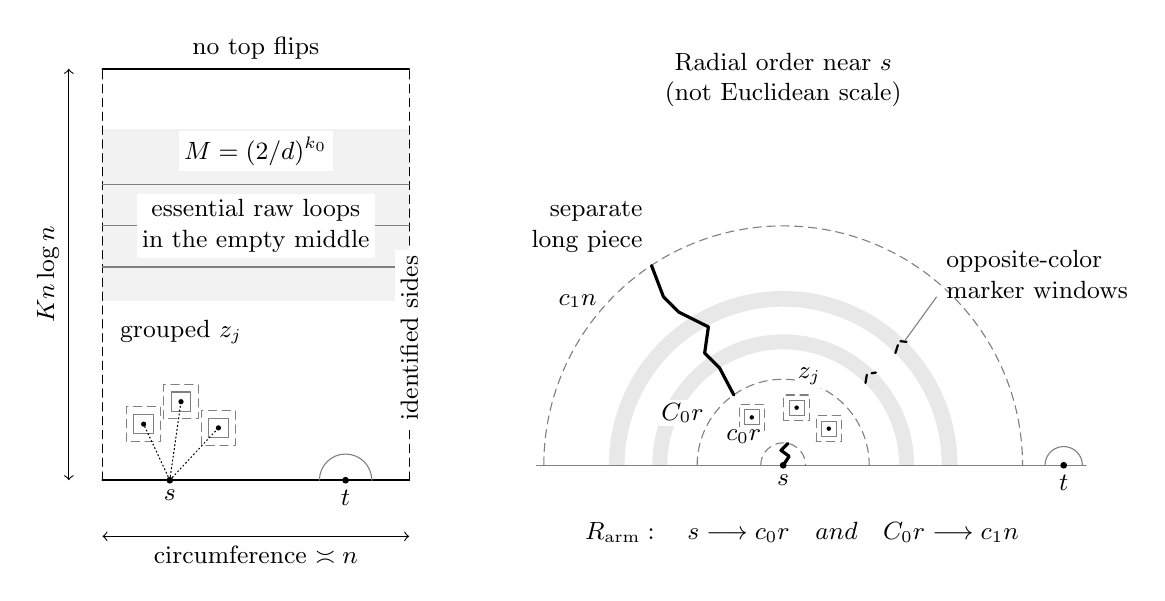
\begin{tikzpicture}[x=.95cm,y=.95cm,font=\small,line cap=round,line join=round]
  \path[fill=gray!10] (0,2.4) rectangle (4.1,4.7);
  \draw[thick] (0,0) -- (4.1,0);
  \draw[thick] (0,5.5) -- (4.1,5.5);
  \draw[densely dashed] (0,0) -- (0,5.5);
  \draw[densely dashed] (4.1,0) -- (4.1,5.5);
  \foreach \y in {2.85,3.4,3.95} {\draw[gray] (0,\y) -- (4.1,\y);}
  \node[fill=white,inner sep=2pt] at (2.05,4.4) {$M=(2/d)^{k_0}$};
  \node[align=center,fill=white,inner sep=2pt] at (2.05,3.4)
    {essential raw loops\\in the empty middle};
  \node[above] at (2.05,5.5) {no top flips};
  \draw[<->] (-.45,0) -- (-.45,5.5);
  \node[rotate=90,above] at (-.45,2.75) {$Kn\log n$};
  \draw[<->] (0,-.75) -- (4.1,-.75);
  \node[below] at (2.05,-.75) {circumference $\asymp n$};
  \fill (.9,0) circle (.045);
  \fill (3.25,0) circle (.045);
  \node[below] at (.9,0) {$s$};
  \node[below] at (3.25,0) {$t$};
  \draw[gray] (2.9,0) arc (180:0:.35);
  \foreach \x/\y in {.55/.75,1.05/1.05,1.55/.7} {
    \draw[gray,densely dashed] (\x-.23,\y-.23) rectangle (\x+.23,\y+.23);
    \draw[gray] (\x-.13,\y-.13) rectangle (\x+.13,\y+.13);
    \fill (\x,\y) circle (.035);
    \draw[densely dotted] (.9,0) -- (\x,\y);
  }
  \node[above] at (1.05,1.7) {grouped $z_j$};
  \node[rotate=90,fill=white,inner sep=2pt] at (4.1,1.9) {identified sides};
  \node[align=center] at (9.1,5.35) {Radial order near $s$\\(not Euclidean scale)};
  \begin{scope}[shift={(9.1,.2)}]
    \foreach \inner/\outer in {1.55/1.75,2.12/2.33} {
      \path[fill=gray!18] (-\outer,0) arc (180:0:\outer)
        -- (\inner,0) arc (0:180:\inner) -- cycle;
    }
    \draw[gray] (-3.3,0) -- (4.05,0);
    \foreach \radius in {.3,1.15,3.2} {
      \draw[gray,densely dashed] (-\radius,0) arc (180:0:\radius);
    }
    \foreach \x/\y in {-.42/.64,.18/.77,.61/.49} {
      \draw[gray,densely dashed] (\x-.17,\y-.17) rectangle (\x+.17,\y+.17);
      \draw[gray] (\x-.1,\y-.1) rectangle (\x+.1,\y+.1);
      \fill (\x,\y) circle (.03);
    }
    \fill (0,0) circle (.045);
    \node[below] at (0,0) {$s$};
    \draw[line width=1.15pt] (0,0) -- (.08,.12) -- (-.03,.2) -- (.06,.29);
    \draw[line width=1.15pt] (-.66,.94) -- (-.85,1.3) -- (-1.05,1.5)
      -- (-1,1.85) -- (-1.4,2.05) -- (-1.6,2.25) -- (-1.76,2.67);
    \draw[densely dashed,thick] (1.1,1.1) -- (1.12,1.22) -- (1.24,1.24);
    \draw[densely dashed,thick] (1.5,1.5) -- (1.55,1.66) -- (1.65,1.65);
    \node[above left,fill=white,inner sep=1pt] at (-.25,.25) {$c_0r$};
    \node[left,fill=white,inner sep=1pt] at (-1.02,.7) {$C_0r$};
    \node[above left,fill=white,inner sep=1pt] at (-2.45,2.06) {$c_1n$};
    \node[above,fill=white,inner sep=1pt] at (.35,1.03) {$z_j$};
    \node[align=left,anchor=west] at (2.05,2.55) {opposite-color\\marker windows};
    \draw[gray] (2.05,2.25) -- (1.63,1.67);
    \node[above left,align=right] at (-1.75,2.72) {separate\\long piece};
    \fill (3.75,0) circle (.045);
    \draw[gray] (3.5,0) arc (180:0:.25);
    \node[below] at (3.75,0) {$t$};
    \node[align=center] at (.25,-.9)
      {$R_{\rm arm}:\quad s\longrightarrow c_0r\quad\text{and}\quad C_0r\longrightarrow c_1n$};
  \end{scope}
\end{tikzpicture}
\caption{The charged cylinder and its two separate arm requirements (schematic, not to scale). The vertical sides in the left panel are identified. Endpoints are grouped at scale $r=n^{1-\varepsilon}$ near $s$, while $t$ is at distance of order $n$; dotted lines are charge strings, not actual paths. The middle observable counts essential raw loops wholly in its strip, not the actual winding cycle used in the later reconstruction event $E$. On the right, the two solid arm pieces need not be connected. The extra opposite-color marker windows lie strictly between radii $2C_0r$ and $c_1n/2$, away from all conditioned cutoff data. Buffers and the finite endpoint configuration are fixed before the mesh limit; omitted distances and radial ratios are not represented metrically.}
\label{fig:charged-cylinder}
\end{figure}


\paragraph{The sign table.}
For a bottom child disk let \(a\in[0,1]\) be the total endpoint
charge in it. Lemma~\ref{physical:winding} gives the following
wrong-expansion numerators, all divided by \(\sin\lambda\):
\begin{equation}\label{physical:charged-table}
 \begin{array}{c|l}
 \text{flips in the child interval}&\text{numerators}\\ \hline
 0&\sin((2-a)\lambda),\quad\sin((1+a)\lambda)\\
 1&\sin(a\lambda)\quad(s),\quad\sin((2-a)\lambda)\quad(t)\\
 2&\sin((3-a)\lambda),\quad\sin(a\lambda).
 \end{array}
\end{equation}
A same-boundary child interval spans less than one period: otherwise
its lift and a period translate cannot be disjoint. Thus each flip
is counted at most once. Top child disks use the zero-flip row.
Contractible wrong-expansion loops have weight
\(2\cos((1-a)\lambda)>0\), and essential loops have weight
\(2\cos(a\lambda)>0\). All entries in the table are nonnegative
except possibly \(\sin((3-a)\lambda)\). In particular, we do not
discard its sign.

Let \(N_j\) count the prescribed local loops at \(z_j\), and
let \(N_t\) count local \(t\)-straddles. Set
\[
 U_\pm=\prod_j u_\pm(a_j)^{N_j},\qquad
 M=(2/d)^{k_0},
\]
where \(k_0\) counts essential closed loops wholly inside an empty
middle strip separated from both ends by enlarged \(O(n)\) bands.
Under either positive cap law, \(M\ge1\) and has polynomial
moments: the strip is covered by \(O(K\log n)\) fixed-ratio
passage bands. Let \(\mathcal T\) be the event of a raw bottom-to-top
through arc. Successive noncontractible actual cycles in separated
transverse bands block such an arc, so Propositions~\ref{prop:routing}
and \ref{prop:screens} give
\begin{equation}\label{physical:through-rarity}
 \PP_\pm(\mathcal T)\le Cn^{-cK}.
\end{equation}
Here \(c>0\) is independent of \(K\). On \(\mathcal T\),
there is no essential closed raw loop and hence \(M=1\).

\paragraph{Local factors and passage errors.}
Let \(Y_\pm\) be the spin integrands relative to their corresponding
positive cap laws. Let \(E\) be the event that the \(s\)-gap
connects actually in its color to a noncontractible cycle near the
bottom, before the middle strip. On \(E\) no child disk cuts off
\(s\), and there is no through arc.  The isolated local factors, relative
to their respective positive cap weights, are
\[
\begin{array}{c|cc}
 \text{local feature}&Y_+&Y_-\\ \hline
 \text{loop around }z_j&u_+(a_j)&u_-(a_j)\\
 s\text{-straddle}&1&0\\
 t\text{-straddle}&1&d\\
 \text{empty-middle essential loop}&2/d&2/d\\
 \text{disk enclosing }s\text{ and all endpoints, not }t&d&1.
\end{array}
\]
The last row covers the intermediate scales between the grouped endpoints
and \(t\); its correct factor is at most one.  The remaining features are
controlled by the passage inventory in the following bounds:
\begin{align}
 |Y_+|&\le M U_+ C^{1+X},\label{physical:correct-majorant}\\
 |Y_-|&\le M U_-d^{N_t}C^{1+X},\label{physical:wrong-majorant}\\
 Y_-&\ge M U_-d^{N_t}C^{-(1+X)}\quad\text{on }E,
 \label{physical:wrong-minorant}
\end{align}
where \(X\) has every fixed exponential moment uniformly in \(n\).
Its passage inventory uses only fixed bottom and top bands,
independently of \(K\), together with the grouped endpoint patch
at scale \(r\).

To prove these bounds, remove locally contained small boundary disks
in descendant order, closing the removed family under descendants.
Their diameters are less than a small fixed fraction of \(n\),
so they contain at most one bottom flip. Lemma~\ref{physical:cap-elimination}
accounts for all neutral cap factors at aggregate passage cost.
In individual cutoff boxes the remaining weights are exactly the
displayed \(u_\pm(a_j)\) loop factors and, at \(t\), the factor
\(d\) for each wrong-expansion local straddle. At \(s\), a local
straddle has wrong weight zero and the correct neutral factor one.

There is one intermediate-scale case which must not be charged once
per scale. A disk enclosing \(s\) and all endpoints but not \(t\)
has correct effective drop \(s-1\), of weight \(d\le1\), and
wrong numerator \(\sin\lambda\), of weight one. These factors
therefore cause no growing error. If inclusion of the endpoint group
disagrees with inclusion of \(s\), the arc crosses a join of length
\(O(r)\) from the gap to that group. A nonlocal such arc gives a
passage across a fixed proportion of the grouped patch or one of its
separated individual patches. The same is true of a nonlocal
contractible loop enclosing endpoints, since it separates them from
the bottom. Cutoff-edge mismatches give the corresponding buffered
patch passages. Genuinely large arcs and essentials outside the
empty middle give passages in the large boundary bands, individually.
Through-arc weights are bounded before cap normalization by a
constant per arc regardless of winding, and each such arc gives a
boundary-band passage.

This is a finite inventory of fixed-shape passage tests at scales
\(r\) and \(n\).  Trim one qualifying portion from each raw arc or loop
in each test.  Distinct raw components have disjoint cut-surface port
incidences, and the fixed number of tests bounds the multiplicity of a
component.  Thus this inventory is bounded by a fixed multiple of the
packing sum of Definition~\ref{angular:passage-packing}, plus a fixed
constant.  Proposition~\ref{prop:passage-moments} supplies all exponential
moments of \(X\). On \(E\), disks
cutting off \(s\) are impossible. The remaining table entries
form a finite strictly positive set, as the charge list is fixed;
the same counting therefore proves the lower bound
\eqref{physical:wrong-minorant}. Notice that \(d^{N_t}\) has been
retained, as is necessary for \(d<1\).

\paragraph{A relative saving for negative terms.}
Off \(\mathcal T\), a nonzero negative integrand requires a
two-flip disk omitting some of the nearby charge: with all charge
included, the first two-flip numerator is \(\sin(2\lambda)>0\).
Let \(B\) denote occurrence of such a disk, and put
\(B_0=B\cap\{Y_-\ne0\}\cap\mathcal T^c\). Its arc intersects a
short join to the endpoint group and travels to distance of order
\(n\). Both colors have actual traversals along its two sides.
Nonzero weight also excludes every pure local \(s\)-straddle below
a sufficiently small multiple of \(r\), forcing a short gap arm.

Choose the constants and buffers of
Corollary~\ref{disk:grouped-cylinder}: the disjoint endpoint annuli lie
between \(c_0r\) and \(C_0r\), and fixed \(0<c_1<c_2\) give an injective
\(s\)-centered half-disk of radius \(c_2n\), separated from the
\(t\)-patch and the middle by positive \(n\)-scale margins.  Its
half-sector between \(c_1n\) and \(c_2n\) has the required fixed ratio
and permitted attachments, counting all bank classes and retaining the
residual-cap condition.  Let \(R_{\rm arm}\)
be the conjunction of an actual gap arm to \(c_0r\) and a separate
same-color traversal from \(C_0r\) to \(c_1n\). The event
\(B_0\) forces these requirements
and also opposite-color traversals in \(J\ge c\log(n/r)-C\)
spaced intermediate marker bands.

Condition on all endpoint-cutoff data, the \(t\)-cutoff data, and
the remote middle-strip states; write this information as
\(\mathcal H\).  Use as the reference in that corollary the fixed flat
cap law and arm cutoff defining \(P(n)\).  The constants above are chosen
so this law agrees with the cylinder graph, odds, and deterministic walls
through \(c_2n\), and its full cutoff lies beyond \(c_1n\) with the
prescribed buffer.  Its reference arm probability is exactly
\(p_{\mathrm{ref}}=e^{P(n)}\); changing to another fixed flat cutoff
would change \(P\) only by \(O(1)\).  That corollary, based on
Lemma~\ref{lem:relative-arm}, gives
\begin{align}
 \PP_-(E\mid\mathcal H)
 &\ge c\,\PP_-(R_{\rm arm}\mid\mathcal H)
 \ge c' p_{\mathrm{ref}}=c'e^P,\label{physical:arm-main}\\
 \PP_-(B_0\mid\mathcal H)
 &\le C(r/n)^\gamma\PP_-(R_{\rm arm}\mid\mathcal H)
 \label{physical:arm-saving}
\end{align}
for a fixed \(\gamma>0\).
For clarity, the first comparison is relative to the two separate
requirements, not an unconditional arm upper bound. Buffered collar
densities compare those requirements under the stated conditioning.
Their supports avoid the conditioned patches. The two measured
blockers can be joined with fixed relative probability through
cleared corridors around the finitely many endpoint boxes at scale
\(r\). Re-search at scale \(n\) then joins this arm to a winding
cycle before the middle, avoiding \(t\). Conversely an ordinary
longer arm forces the two requirements, giving the second lower
bound. In each marker window the conditional same-color scaffold
preserves the required traversal while making a wall-to-wall screen
which prevents the opposing marker traversal. Thus each additional
opposite marker costs a factor at most \(1-c\), relative to the
traversal requirement and with the separated short arm carried along.
Iteration over \(J\) bands proves \eqref{physical:arm-saving}.

\paragraph{Comparison of the two expansions.}
The positive factor \(W=M U_-d^{N_t}\) is measurable with respect
to \(\mathcal H\).  Multiplying the two conditional inequalities by
\(W\) and averaging gives the relative comparison
\begin{equation}\label{physical:weighted-saving}
 \EE_-[W\one_{B_0}]
 \le \frac Cc(r/n)^\gamma\EE_-[W\one_E].
\end{equation}
Thus the negative contribution is compared to the same main event with
its full weight \(d^{N_t}\), even on states where that factor is small.
The bounded cutoff comparisons then give
\begin{equation}\label{physical:main-mass}
 \EE_-[W\one_E]\ge
 c(\EE_-M)e^{P+D_*}\prod_jF_-(a_j;r).
\end{equation}
Before passage errors, \eqref{physical:weighted-saving} makes the bad
contribution smaller than this main mass by the fixed power
\(n^{-\gamma\varepsilon}\).
On the through event, \(M=1\). Its upper bound uses only the fixed
feature bands, whose polynomial moment exponents do not depend on
\(K\). H\"older's inequality and
\eqref{physical:through-rarity} therefore make its absolute
contribution negligible after choosing a sufficiently large fixed
\(K\). The main mass has an inverse-polynomial lower bound whose
exponent does not depend on \(K\), since \(M\ge1\).

Now hold \(K\) and \(\varepsilon\) fixed. The absorption rule
removes the factors \(C^{\pm(1+X)}\) at an arbitrarily small power
cost. Choose that power smaller than the saving in
\eqref{physical:arm-saving}; the negative and through errors remain
negligible. Off these errors the wrong expansion is nonnegative,
and \eqref{physical:wrong-minorant} supplies its positive main part.
For every sufficiently small \(\eta>0\), increasing constants
if necessary, equality of the two tensor expansions consequently
implies
\[
 Z_-^{\rm cap}(\EE_-M)e^{P+D_*}\prod_jF_-(a_j;r)
 \le C_{\eta,\varepsilon,K}n^\eta
 Z_+^{\rm cap}(\EE_+M)\prod_jF_+(a_j;r).
\]
Here the correct upper bound follows from
\eqref{physical:correct-majorant}, the same separated-patch
comparisons, and absorption. All local lower baselines are inverse
polynomials, so the same argument applies to this upper comparison.

Repeat with both wire polarities reversed on the identical cylinder,
using the same strings, cutoffs, drops, and middle observable \(M\).
The two cap laws are interchanged. Their partition and middle-mean
ratios therefore cancel exactly on multiplication. Local costs in
the two designations differ by \(O(1)\). Taking logarithms gives
\[
 P+D_*+\sum_j\log\frac{F_-(a_j;r)}{F_+(a_j;r)}
 \le o(\log n).
\]
Finally \eqref{physical:cutoff-increment} changes \(r\) to \(n\)
at cost \(O(\varepsilon\log n+1)\). Given any final tolerance,
choose \(\varepsilon\) first sufficiently small and then make the
absorption tolerance smaller still. This proves
\eqref{physical:charge-budget}.
\end{proof}
